\section{Introduction\label{bso_sec:intro}}
% ====================

\begin{figure}[!htp]
\begin{center}
\begin{ccTexOnly}
  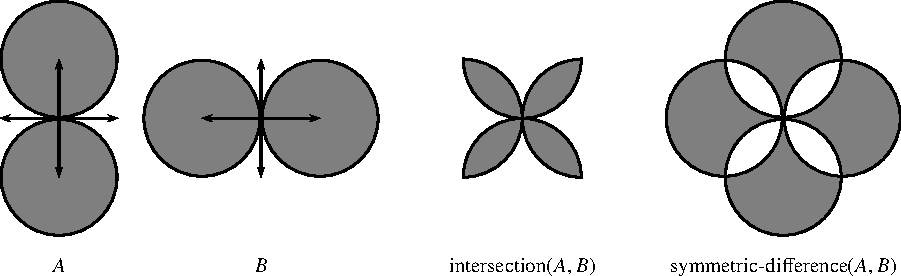
\includegraphics{Boolean_set_operations_2/fig/teaser}
\end{ccTexOnly}
\label{fig:teaser}
\begin{ccHtmlOnly}
  <p><center>
    <img src="./fig/teaser.gif" border=0 alt="Boolean Set-Operations">
  </center>
\end{ccHtmlOnly}
\caption{Examples of Boolean set-operations on general polygons.} 
\end{center}
\end{figure}

This package consists of the implementation of Boolean set-operations
on point sets bounded by weakly $x$-monotone curves\footnote{A continuous
planar curve $C$ is {\em weakly $x$-monotone} if every vertical line intersects it at
most once, or if it is vertical. Hereafter we refer to weakly $x$-monotone curves as  $x$-monotone curves.} in 2-dimensional Euclidean space. In particular,
it contains the implementation of {\em regularized} Boolean set-operations,
intersection predicates, and point containment predicates.
Figure~\ref{fig:teaser} shows simple examples of such operations.

Ordinary Boolean set-operations, which distinguish between the
interior and the boundary of a polygon, are not implemented within this
package. The \ccc{Nef_2} package supports these operations for (linear)
polygons; see Chapter~\ref{chap:nef_2}.

In the rest of this chapter we use, unless otherwise stated, the
traditional notation to denote regularized operations; e.g., $P \cap Q$
means the {\em regularized} intersection of $P$ and $Q$.

Our package supports the following Boolean set-operations on two point
sets $P$ and $Q$ that each is the union of one or more general polygons:
\begin{description}
\item[Intersection] computes the intersection $R = P \cap Q$.
\item[Join] computes the union $R = P \cup Q$.
\item [Difference] computes the difference $R = P \setminus Q$.
\item [Symmetric Difference] computes the symmetric
  \ccHtmlNoLinksFrom{difference} $P = P \oplus Q = (P \setminus Q) \cup (Q \setminus P)$.
\item[Complement] computes the complement
  \lcTex{$R = \overline{P}$.}
  \lcRawHtml{<i>R = <span style="text-decoration: overline;">P</span>.</i>}
\item [Intersection predicate] tests whether the two sets $P$ and $Q$
  overlap, distinguishing three possible scenarios: (i) the two sets
  intersect on their interior (that is, their regularized intersection
  is not empty $P \cap Q \neq \emptyset$); (ii) the boundaries of two
  sets intersect but their interiors are disjoint; namely they have a
  finite number of common points or even share a boundary curve (still
  in this case $P \cap Q = \emptyset$; and (iii) the two sets are
  disjoint.
\end{description}
In general, the set $R$, resulting from a regularized Boolean
set-operation, is considered as being a closed point-set; see definition of regularized boolean set operations below.

In the rest of this chapter we review the Boolean set-operations package
in more depth. In Section~\ref{bso_sec:bso_lin} we focus on Boolean 
set-operations on linear polygons, introducing the notion of polygons with 
holes and of a general polygon set. Section~\ref{bso_sec:bso_gen}
introduces general polygons.
We first discuss polygons whose edges are either line segments or circular
arcs and then explain how to construct and use general polygons whose edges
can be arbitrary weakly $x$-monotone curves.
